%%%%%%%%%%%%%%%%%%%%%%%%%%%%%%%%%%%%%%%%%%%%%%%%%%%%%%%%%%%%%%%%%%%%%%%%%%%%%%%
% Beginn des Abstrakts
%%%%%%%%%%%%%%%%%%%%%%%%%%%%%%%%%%%%%%%%%%%%%%%%%%%%%%%%%%%%%%%%%%%%%%%%%%%%%%%
\addcontentsline{toc}{chapter}{Summary}
%
{\large \textbf{\textsf{Summary}}}
\vspace*{3em}

Sorption equilibrium data are fundamental to design and develop sorption systems. Currently, some databases exist which contain experimental equilibrium data, e.g., Springer Materials, NIST, Dortmund Data Bank. However, no open-source database exists containing both experimental sorption equilibrium data as well as generalized equilibrium models and the associated coefficients of sorption working pairs.

Here, the sorption property library – SorpPropLib – comes in. SorpPropLib contains generalized equilibrium models, associated coefficients of adsorption and absorption working pairs, and experimentally measured equilibrium data. The working principle of SorpPropLib is explained below.

\textbf{Working principle of SorpPropLib}

The equilibrium models are implemented in \textit{C}, and the coefficients and experimental data are stored text-based in a \textit{JSON database}. First, a sorption work pair object is initialized by specifying a sorption work pair, including the equilibrium and refrigerant model. Then, the user can calculate various sorption equilibrium data using the sorption working pair object. The schematic of the working principle is shown below.
%
\begin{figure}[!htp]
	{\noindent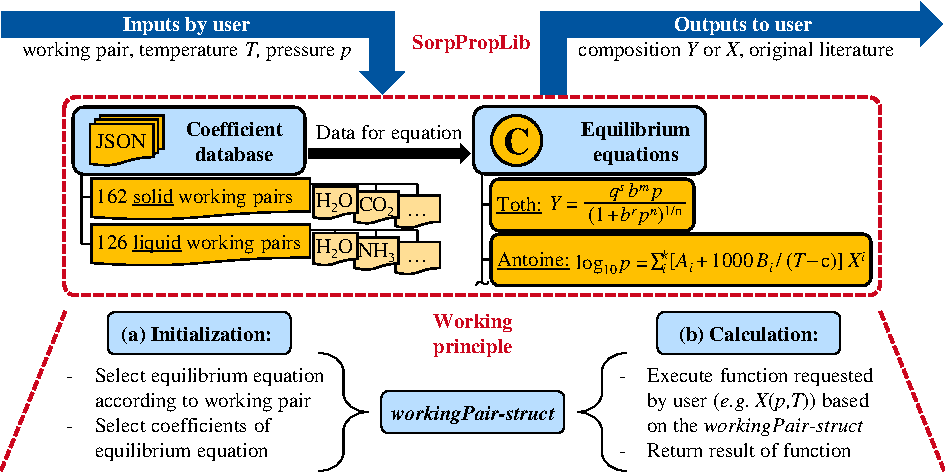
\includegraphics[width=\textwidth, keepaspectratio]{figs/workflow.pdf}}
\end{figure}

\textbf{Integration of SorpPropLib into other programming environments}

SorpPropLib can currently be used from 6 programming environments besides the programming language \textit{C}: \textit{C++}, \textit{Python}, \textit{Matlab}, \textit{Modelica}, \textit{LabVIEW}, and \textit{Excel}. For this purpose, SorpPropLib is compiled as a dynamic link library (DLL) and integrated into the programming environments via wrapper functions. In addition, some of the programming environments (e.g., \textit{Python}) contain functions for visualizing equilibrium data and creating or reading out the \textit{JSON database}. The scheme of integrating SorpPropLib into other programming environments is shown below.
%
\begin{figure}[!htp]
	{\noindent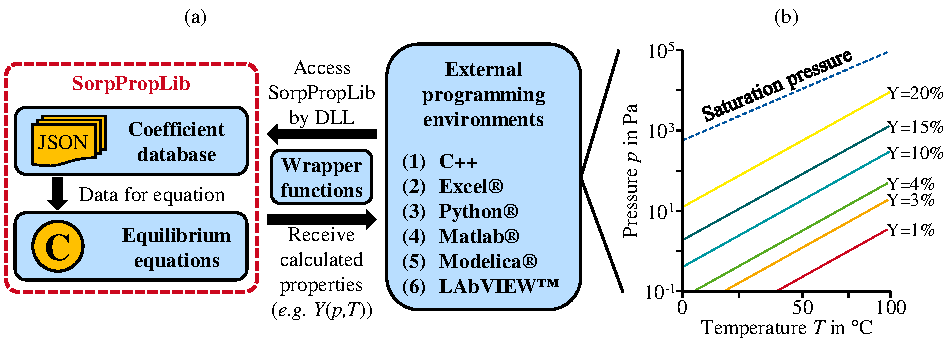
\includegraphics[width=\textwidth, keepaspectratio]{figs/prog_environments.pdf}}
\end{figure}

\textbf{Citing SorpPropLib}

The SorpPropLib shall be cited via the following journal article:

Yang, Zhiyao; Gluesenkamp, Kyle R.; Frazzica, Andrea (2021): Equilibrium vapor pressure properties for absorbent and adsorbent materials. In: \textit{International Journal of Refrigeration} 124, pp. 134-166. DOI: 10.1016/j.ijrefrig.2020.12.013.

Furthermore, the following conference paper shall be cited when using the \textit{JSON database}, \textit{C} code, or an interface to the programming environments mentioned before:

Engelpracht, M.; Yang, Z.; Gluesenkamp, K. R.; Turnaoglu, T.; Seiler, J.; Bardow, A. (2020): SorpPropLib: An Open-Source Database for Sorption Equilibrium Properties. In: \textit{ISHPC 2021 proceedings - online pre-conference 2020}, pp. 33-36. International Sorption Heat Pump Conference. Berlin, Germany.

%
\cleardoublepage
%%%%%%%%%%%%%%%%%%%%%%%%%%%%%%%%%%%%%%%%%%%%%%%%%%%%%%%%%%%%%%%%%%%%%%%%%%%%%%%